\chapter{Extended phase model \label{chap:exphsmodel}}

In Chapter~\ref{sec:partialtracking} techniques were presented for discovering
partials in a signal. Each partial is a set of analysis points indexed by time.
The information at each analysis point can be used to synthesize a portion of
the partial and these are combined to give a signal representing a partial.
The various techniques to synthesize these pieces of the signal discussed here
differ in the orders used for analysis and those for synthesis. The first
technique presented simply synthesizes signals of short duration using the
estimated parameters and blends these segments together. We recognize that
having multiple estimations of parameters at discrete times within the partial
duration allow us to postulate, via interpolation, functions describing the
partial of higher order than those whose parameters were estimated during
analysis. It is shown that this strategy is not always to our advantage ---
interpolants of higher order than the underlying function can suffer from errors
due to over-fitting. In the case of functions that are always better
approximated by higher order polynomials, we will see that there is an advantage
to using high order interpolation. These cases are illustrated through the
analysis and synthesis of synthetic signals.

\section{Partial synthesis \label{sec:partialsynthesis}}

A popular technique for synthesizing partials from a set of analysis points is
the \textit{overlap-and-add} procedure \cite{portnoff1976implementation},
\cite{moore1990elements}. We assume that in the neighbourhood of $\tau_{r}$ the
partial's signal is approximately described by the function $x(n) \approx
f_{\tau_{r}}(n-\tau_{r})$. To synthesize an approximation of $x$ we sum windowed
$f_{\tau_{r}}$ at multiple locations, windowed by a function $w$ with finite
support so the resulting signal has finite energy and the piecewise assumption
is maintained. For simplicity we assume the $\tau_{r}$ are equally spaced by $H$
samples, and $\tau_{0}=0$, so we have $\tau_{r} = rH$. The length of the window
function $w$ is $M = VH + 1$ samples, with $V,H \in \mathbb{N}%
$\footnote{%
    $M$ is always odd so one may wonder how the Fast Fourier Transform can be
    used to invert $F_{\tau_{r}}$, the frequency domain representaion of
    $f_{\tau_{r}}$.  Recall that the DTFT can be interpreted as the coefficients
    of a Fourier series that give the periodic version of the analysed signal.
    Also recall that we use window functions that are real and even. In practice
    the edges of the window are often equal to zero so that the length of the
    non-zero part is equal to the length of the DTFT $N$. In the case they are
    not, simply ensuring that values in the window indexed by integer multiples
    of $N$ are 0, and that the value at the centre of the window is 1 will ensure proper
    synthesis \cite[p.~244]{portnoff1976implementation}. In that case, the values
    outside of the part of the window presented to the DTFT are folded into this
    region using the window indices modulo-$N$. See
    \cite{portnoff1976implementation} and \cite{moore1990elements} for more details on this
    procedure.%
}.
The approximate signal at sample $n$ is then
\[
    \tilde{x}(n) = \sum_{l=L_{-}}^{L^{+}} w(n-lH) f_{\tau_l}(n-\tau_l)
\]
where
\[
    L_{-} = \left\lceil \frac{n}{H} \right\rceil - V
\]
and
\[
    L_{+} = \left\lfloor \frac{n}{H} \right\rfloor + V
\]
This method has some drawbacks. Usually the function $f$ is an approximation
$\tilde{f}$ of the true underlying function. In the case of partial tracking,
often partials that are too short are discarded or missed. At amplitude
transients, these short partials are important for reproducing sharp attacks
that are shorter than the window length. If these partials are missing, the
resulting signal takes on a transient similar to the window shape. This could be
overcome by choosing a window with a shape similar to the overall amplitude
envelope in the attack region when resynthesizing an attack transient.

Another drawback is that no attempt is made to interpolate between the functions
estimated at $\tau_{r}$ and $\tau_{r+1}$ using the model that the underlying
sinusoids are non-stationary\footnote{%
    This is one of the causes of ``pre-echo'' when
    time-stretching using the STFT \cite{roebel2003transient}.%
}
From Equation~\ref{eq:ddmsyseq} we know we can estimate a polynomial of
arbitrary order for phase. We will see that using this additional information
can give us an interpolating function closer to the underlying model.

\section{The interpolating analysis-synthesis system}

In the following, we investigate the synthesis quality of three interpolating
analysis-synthesis systems. The qualifier ``interpolating'' is used because each
system takes the multiple sets of estimated parameters of a smaller order model
and interpolates them with a higher oder model, which is then used for
synthesis. The systems will be denoted $\mathscr{S}_{p,q}$ where $p$ is the
order of the analysis system and $q$ the order of the synthesis system, e.g., a
linear analysis system has $p=1$, etc.

\section{$\mathscr{S}_{1,3}$: the McAulay-Quatieri method}

\subsection{Analysis: linear phase \label{sec:S13analysis}}

For the McAulay-Quatieri method, the model is a sinusoid of constant frequency
(linear phase) in each analysis frame. To estimate the frequency of this
sinusoid we find the bin with the most energy and find a refined estimate of the
frequency as the maximum of a quadratic interpolating polynomial fit to this bin
and its two neighbouring bins. This is a procedure documented in
\cite[p.~45]{serra1989system}. The interpolation is best performed in the
log-spectrum and on a spectrum produced using a window, such as a zero-padded
Hann window, giving a wide enough main-lobe so that the three points lie on this
lobe and not on side-lobes. A refined estimate of the amplitude of the sinusoid
is obtained with this procedure as well.

In the original paper by McAulay and Quatieri, they do not use this technique
but, as they show an example analysis of a speech signal, instead adjust the
analysis window to be a multiple of the period of the glottal pulse. The bins of
the DTFT used in the analysis will be integer multiples of the frequency given
as the reciprocal of this period. Under the model of the speech signal as
harmonically related sinusoids, the best estimate for the frequency is the bin
of a local maximum, its amplitude the modulus of the spectrum at this maximum, and
the phase the argument.

In our system, we use a fixed window size. To estimate the phase then we use
Equation~\ref{eq:ddmestc0} with
\[
    \gamma_{\text{MQ}}(n)=\exp(2\pi\frac{k^{\ast}}{M}n)
\]
where $k^{\ast}$ is the bin we have determined to correspond to the frequency of
the sinusoid. The inital phase is then $\Im \left\{ c_{0} \right\}$.

\subsection{Synthesis: cubic phase \label{sec:S13synthesis}}

Given two local maxima of the
DTSTFT $X(\tau_0,\omega_0)$ and $X(\tau_1,\omega_1)$, where $H = \tau_1 -
\tau_0$ we can conjecture a cubic
polynomial phase function for the imaginary part of the phase argument

\begin{equation}
    \tilde{\phi}(n) = \Im\left\{c_3\right\} (n-\tau_0)^3 + \Im\left\{c_2\right\} (n-\tau_0)^2 + \Im\left\{c_1\right\} (n-\tau_0) + \Im\left\{c_0\right\}
\end{equation}

By noting that we have 2 measurements of the phase and frequency,
$\angle\{X(\tau_0,\omega_0)\}$ and $\angle\{X(\tau_1,\omega_1)\}$, and the frequency
is the derivative of the phase, we can solve for the coefficients of the
polynomial phase function using the following linear system of equations,
assuming the DTSTFT was computed using a real and even window
\begin{equation}
    \begin{pmatrix}
        0   & 0     & 0 & 1 \\
        H^3 & H^2   & H & 1 \\
        0   & 0     & 1 & 0 \\
        3 H^2 & 2 H & 1 & 0
    \end{pmatrix}
    \begin{pmatrix}
        \Im\{c_3\} \\
        \Im\{c_2\} \\
        \Im\{c_1\} \\
        \Im\{c_0\}
    \end{pmatrix}
    =
    \begin{pmatrix}
        \angle\{X(\tau_0,\omega_0)\} \\
        \angle\{X(\tau_1,\omega_1)\} + 2 \pi M \\
        \omega_0 \\
        \omega_1        
    \end{pmatrix}
\end{equation}
We choose $M$ so that
\begin{equation}
    \label{eq:minfmmq}
    \int_{0}^{H}(\frac{d^{2}\tilde{\phi}}{dt^2}(t))^{2}dt
\end{equation}
is minimized in order to have a smooth evolution of phase in the interpolated
region. $M$ is necessary because some integer number of periods of a sinusoid
will have passed from times $\tau_{0}$ to $\tau_{1}$. Informally we choose $M$
so that a polynomial describing the phase evolution between these two times
takes a direct route, which is a plausible criterion because a signal with more
radical phase variation would unlikely exhibit a spectrum that could be well
described by two points in the time-frequency plane, i.e., the signal
would exhibit a large bandwidth. See \cite[p.~751]{mcaulay1986speech} for
further clarification.

As only two measurements of the amplitude of the sinusoid are available,
$|X(\tau_0,\omega_0)|$ and $|X(\tau_1,\omega_1)|$, the coefficients
$c_3$ and $c_2$ are purely imaginary and the real parts of $c_1$ and $c_0$ are
determined as
\begin{equation}
    \begin{pmatrix}
        0 & 1 \\
        H & 1
    \end{pmatrix}
    \begin{pmatrix}
        \Re\{c_1\} \\
        \Re\{c_0\}
    \end{pmatrix}
    =
    \begin{pmatrix}
        \log(|X(\tau_0,\omega_0)|) \\
        \log(|X(\tau_1,\omega_1)|)
    \end{pmatrix}
\end{equation}

\section{$\mathscr{S}_{2,3}$ and $\mathscr{S}_{2,5}$: the DDM-based methods}

Here we extend the $\mathscr{S}_{1,3}$ model of McAulay-Quatieri to account for
the additional parameters estimated via the DDM. For the $\mathscr{S}_{2,3}$
model, we must introduce additional constraints into the system as we have more
estimated parameters than are available in the synthesis model. It would be
possible to solve this system via least-squares, but the proposed constraints
simplify analytically the expression maximizing the smoothness of the phase
function, and give satisfactory results. For the $\mathscr{S}_{2,5}$ model the
derivation is straightforward as in the $\mathscr{S}_{1,3}$ case --- there are
the same number of estimated parameters as there are parameters in the model.

\subsection{Analysis: quadratic phase \label{sec:s235analysis}}

The DDM is used on segments of the signal to estimate the parameters of sinusoid
with a complex quadratic phase polynomial. This sinusoid has the form
\begin{equation}
    \label{eq:quadraticphasepoly}
    x_{a}(n) = \exp \left(a_2 n^{2} + a_1 n + a_0 \right)
\end{equation}
with $a_{i} \in \mathbb{C}$.

We can estimate the coefficients of Equation~\ref{eq:quadraticphasepoly} using
the DDM. We write Equation~\ref{eq:ddmsyseq} in matrix form with $Q=2$
\begin{equation}
    \begin{pmatrix}
        \left\langle \mathcal{T}^{0} x , \overline{\psi}_{1} \right\rangle &
        2\left\langle \mathcal{T}^{1} x , \overline{\psi}_{1} \right\rangle \\
        \vdots & \vdots \\
        \left\langle \mathcal{T}^{0} x , \overline{\psi}_{R} \right\rangle & 
        2\left\langle \mathcal{T}^{1} x , \overline{\psi}_{R} \right\rangle
    \end{pmatrix}
    \begin{pmatrix}
        a_{1} \\
        a_{2}
    \end{pmatrix}
    =
    \begin{pmatrix}
        -\left\langle  x , \frac{d\overline{\psi}_{1}}{dn} \right\rangle \\
        \vdots \\
        -\left\langle  x , \frac{d\overline{\psi}_{R}}{dn} \right\rangle
    \end{pmatrix}
\end{equation}

From this we recognize we need to define three functions
\begin{equation}
    \left\langle \mathcal{T}^{0} x , \overline{\psi}_{k} \right\rangle 
    =
    \sum_{m=0}^{M-1} w(m) x(m + \tau) \exp(-j 2 \pi \frac{k m}{M})
\end{equation}
\begin{equation}
    \left\langle \mathcal{T}^{1} x , \overline{\psi}_{k} \right\rangle
    =
    \sum_{m=0}^{M-1} m w(m) x(m + \tau) \exp(-j 2 \pi \frac{k m}{M})
\end{equation}
\begin{equation}
    \left\langle  x , \frac{d\overline{\psi}_{k}}{dn} \right\rangle
    =
    -j 2 \pi \frac{k}{M} X_{p_{1}} \left( \tau , k \right) + 
    \sum_{m=0}^{M-1} \frac{dw}{dn}(m) x(m + \tau) \exp(-j 2 \pi \frac{k m}{M})
\end{equation}
Where $M$ is the length of the window and $k$ is the frequency
``bin''\footnote{For tractability, the functions $X(\tau,k)$ are only evaluated at
    a finite number of frequencies, which are often called ``bins'' in the
signal processing literature.}. We also
only consider $x$ at the samples $m = [0, \dotsc, M-1]$ because we can always
shift the time reference to view an arbitrary contiguous segment of signal with
these indices.

We then find $k^{\ast}$ such that $X$ is maximum. If multiple components
are present in the signal and are sufficiently separated in frequency, we can
split the signal up into frequency bands and find local maxima. A technique for
doing so is described in \cite[p.~42]{serra1989system}. To have a system of
equations with a unique solution, we take the two adjacent bins $k-1$ and $k+1$
to have enough unique atoms for Equation~\ref{eq:ddmsyseq}. These bins should
only contain energy from the component whose parameters we are interested in
measuring --- this is true if the components are adequately separated in time
and frequency. We could choose only two bins to have a non-singular system, and
there are many possibilities for choosing different atoms
\cite[p.~4639]{betser2009sinusoidal}. We choose three from the same frame to
have improved estimation accuracy in situations where components are adaquately
separated in frequency, while avoiding a more sophisticated local peak selection
procedure. Then $a_2$ and $a_1$ can be determined by solving the linear system
\begin{equation}
    \begin{pmatrix}
        \left\langle \mathcal{T}^{0} x , \overline{\psi}_{k-1} \right\rangle &
        \left\langle \mathcal{T}^{1} x , \overline{\psi}_{k-1} \right\rangle \\
        \left\langle \mathcal{T}^{0} x , \overline{\psi}_{k} \right\rangle &
        \left\langle \mathcal{T}^{1} x , \overline{\psi}_{k} \right\rangle \\
        \left\langle \mathcal{T}^{0} x , \overline{\psi}_{k+1} \right\rangle & 
        \left\langle \mathcal{T}^{1} x , \overline{\psi}_{k+1} \right\rangle
    \end{pmatrix}
    \begin{pmatrix}
        a_{1} \\
        2a_{2}
    \end{pmatrix}
    =
    \begin{pmatrix}
        -\left\langle  x , \frac{d\overline{\psi}_{k-1}}{dn} \right\rangle \\
        -\left\langle  x , \frac{d\overline{\psi}_{k}}{dn} \right\rangle \\
        -\left\langle  x , \frac{d\overline{\psi}_{k+1}}{dn} \right\rangle
    \end{pmatrix}
\end{equation}
With $a_{1}$ and $a_{2}$ determined, we can use Equation~\ref{eq:ddmestc0} to
estimate $a_0$. We will write $a^{\tau}_{i}$ to refer to coefficient $i$
determined at time $\tau$.

\subsection{Synthesis: cubic order ($\mathscr{S}_{2,3}$)
\label{sec:s23synthesis}}

In this section we describe how to obtain a cubic phase polynomial from
local estimations of the coefficients of a quadratic phase polynomial.

\subsubsection{The phase part}

A complex sinusoid with cubic phase has the following form:
\begin{equation}
    \label{eq:cubicphasepoly}
    \beta(n) = \exp \left(j\left(b_3 n^{3} + b_2 n^{2} + b_1 n + b_0
        \right)\right)
\end{equation}
with $b_{i} \in \mathbb{R}$. This sinusoid has magnitude 1 everywhere, only its
phase is changing.

Once the $\boldsymbol{a}^{\tau}$ have been determined
at two times $\tau_{0}$ and $\tau_{1}$, with $H = \tau_{1} - \tau_{0}$, and these
times have between determined as connected (see
Chapter~\ref{chap:partialtracking}), we can write a system of equations
to determine an interpolating cubic phase polynomial. To avoid numerical
instabilities and for simplicity, we shift the time origin so that $\tau_{0} =
0$. This means $b_0 = \Im \left\{ a^{\tau_0}_{0} \right\}$. To reduce the size
of the system, we require that 
\[
    \frac{d \phi}{d n} \left(\frac{H}{2} \right)
    =
    \frac{1}{2}
    \left( \Im \left\{ a^{\tau_0}_{1} \right\} + \Im \left\{ a^{\tau_1}_{1}
    \right\} \right)
\]
and
\[
    \frac{d^{2} \phi}{d n^{2}} \left(\frac{H}{2}
    \right)
    =
    \frac{1}{2} \left( \Im \left\{ a^{\tau_0}_{2} \right\} + \Im \left\{
    a^{\tau_1}_{2} \right\} \right)
\]
i.e., the frequency and first-order frequency modulation in the middle of the
segment are the average of the two measured coefficients. Finally we require the
that the change in phase from time $0$ to $H$ correspond to that what was
observed, but account for the cycles that were not observed by adding an integer
number of $2\pi$ radians. If $\phi(n)=j(b_3 n^{3} + b_2 n^{2} + b_1 n + b_0)$,
then
\[
    \phi \left( H \right)
    =
    \Im \left\{ a^{\tau_1}_{0} \right\} - \Im \left\{ a^{\tau_0}_{0} \right\}
    + 2 \pi U^{\ast}
\]
where $U^{\ast} \in \mathbb{Z}$ is determined to minimize
Equation~\ref{eq:minfmmq}, in this case:
\begin{equation}
    \label{eq:minfmcubic}
    \tilde{U} = \argmin_{U} \int_{0}^{H} \left(
    6 b_3 t + 2 b_2 \right)^{2} dt
\end{equation}
which is then rounded to the nearest integer to give $U^{\ast}$. To summarize we have
\begin{equation}
    \begin{pmatrix}
        H^{3} & H^{2} & H \\
        \frac{3}{4}H^{2} & H & 1 \\
        3 H & 2 & 0
    \end{pmatrix}
    \begin{pmatrix}
        b_{3} \\
        b_{2} \\
        b_{1}
    \end{pmatrix}
    =
    \begin{pmatrix}
        \Im \left\{ a^{\tau_1}_{0} \right\} - \Im \left\{ a^{\tau_0}_{0} \right\}
            + 2 \pi U^{\ast} \\
        \frac{1}{2}
        \left( \Im \left\{ a^{\tau_0}_{1} \right\} + \Im \left\{ a^{\tau_1}_{1}
        \right\} \right) \\
        \frac{1}{2} \left( \Im \left\{ a^{\tau_0}_{2} \right\} + \Im \left\{
        a^{\tau_1}_{2} \right\} \right)
    \end{pmatrix}
\end{equation}
Solving for $b_1, \dotsc, b_3$, we have
\[
    \begin{pmatrix}
        b_{3} \\
        b_{2} \\
        b_{1}
    \end{pmatrix}
    =
    \begin{pmatrix}
        \frac{4}{H^3} \left( \Im \left\{ a^{\tau_1}_0 \right\}
            - \Im \left\{ a^{\tau_0}_0 \right\} + 2 \pi U^{\ast} \right)
        - \frac{2}{H^{2}} \left( \Im \left\{ a^{\tau_1}_1 \right\}
            + \Im \left\{ a^{\tau_0}_1 \right\} \right) \\
        \frac{-6}{H^2} \left( \Im \left\{ a^{\tau_1}_0 \right\}
            - \Im \left\{ a^{\tau_0}_0 \right\} + 2 \pi U^{\ast} \right)
        - \frac{3}{H} \left( \Im \left\{ a^{\tau_1}_1 \right\}
            + \Im \left\{ a^{\tau_0}_1 \right\} \right)
        + \frac{1}{4}  \left( \Im \left\{ a^{\tau_0}_{2} \right\} + \Im \left\{
            a^{\tau_1}_{2} \right\} \right) \\
        \frac{-H}{4}  \left( \Im \left\{ a^{\tau_0}_{2} \right\} + \Im \left\{
            a^{\tau_1}_{2} \right\} \right) 
        + \frac{3}{H} \left( \Im \left\{ a^{\tau_1}_0 \right\}
            - \Im \left\{ a^{\tau_0}_0 \right\} + 2 \pi U^{\ast} \right)
        -  \Im \left\{ a^{\tau_1}_1 \right\}
            - \Im \left\{ a^{\tau_0}_1 \right\}
    \end{pmatrix}
\]
and then $\tilde{U}$ is determined using Equation~\ref{eq:minfmcubic} to be
\[
    \tilde{U} = \frac{1}{4 \pi} \left[ H \left( \Im \left\{ a^{\tau_1}_1
            \right\} + \Im \left\{
        a^{\tau_0}_1 \right\} \right)
        -2 \left( \Im \left\{ a^{\tau_1}_0 \right\} - \Im \left\{
        a^{\tau_0}_0 \right\} \right) \right]
\]
and then rounded to obtain $U^{\ast}$.

\subsubsection{The amplitude part}

Solving for the cubic polynomial describing the local amplitude function
\begin{equation}
    \mu(n) = \exp \left(c_3 n^{3} + c_2 n^{2} + c_1 n + c_0 \right)
\end{equation}
with $c_i \in \mathbb{R}$, is more straightforward analytically as it does not
require solving to maximize the smoothness of resulting polynomial. To require
continuity at the end-points of our polynomial, we require
\[
    \mu(0) = \Re \left\{ a^{\tau_0}_0 \right\}
\]
and
\[
    \mu(H) = \Re \left\{ a^{\tau_1}_0 \right\}
\]
The first constraint is satisfied simply by setting $c_0 = \Re \left\{
a^{\tau_0}_0 \right\}$. The second will be accounted for in a constrained
least-squares solution for the other coefficients. The other observations are
\[
    \frac{d \mu}{dn} (0) = \Re \left\{ a^{\tau_0}_1 \right\}
\]
\[
    \frac{d \mu}{dn} (H) = \Re \left\{ a^{\tau_1}_1 \right\}
\]
\[
    \frac{d^2 \mu}{dn^2} (0) = \Re \left\{ a^{\tau_0}_2 \right\}
\]
\[
    \frac{d^2 \mu}{dn^2} (H) = \Re \left\{ a^{\tau_1}_2 \right\}
\]
The constrained least-squares problem to be solved is then
\begin{equation}
    \begin{pmatrix}
        0 & 0 & 1 \\
        3 H^2 & 2 H & 1 \\
        0 & 2 & 0 \\
        6 H & 2 & 0
    \end{pmatrix}
    \begin{pmatrix}
        c_3 \\
        c_2 \\
        c_1
    \end{pmatrix}
    =
    \begin{pmatrix}
        \Re \left\{ a^{\tau_0}_1 \right\} \\
        \Re \left\{ a^{\tau_1}_1 \right\} \\
        \Re \left\{ a^{\tau_0}_2 \right\} \\
        \Re \left\{ a^{\tau_1}_2 \right\}
    \end{pmatrix}
\end{equation}
subject to
\[
    \begin{pmatrix}
        H^3 & H^2 & H
    \end{pmatrix}
    \begin{pmatrix}
        c_3 \\
        c_2 \\
        c_1
    \end{pmatrix}
    =
    \begin{pmatrix}
        \Re \left\{ a^{\tau_1}_0 \right\}
    \end{pmatrix}
\]
This can be solved using numerical methods, in particular, using a specific
interpretation of weighted least-squares \cite[p.~266]{golub1996matrix}.

\subsection{Synthesis: quintic order ($\mathscr{S}_{2,5}$) \label{s25synthesis}}

\subsubsection{The phase part}

Solving for the coefficients of a quintic phase polynomial is done very
similarly to Section~\ref{sec:s23synthesis}. As we have the same number of
analysed parameters and synthesis parameters, no constraints have to be
introduced to solve the system apart from the value $U$ that maximizes
smoothness of the phase function. The quintic phase polynomial is%
\footnote{Remember, this sinusoid has constant amplitude of 1 and
this function only describes its change of phase.}
\begin{equation}
    \label{eq:quinticphasepoly}
    \lambda(n) = \exp \left(j\left(u_5 n^{5} + u_4 n^{4} + u_3 n^{3} + u_2 n^{2}
    + u_1 n + u_0 \right)\right)
\end{equation}
with $u_i \in \mathbb{R}$. We have
\[
    \phi(0) = \Im \left\{ a^{\tau_0}_0 \right\}
\]
\[
    \frac{d \phi}{d n}(0) = \Im \left\{ a^{\tau_0}_1 \right\}
\]
\[
    \frac{d^{2} \phi}{d n^{2}}(0) = \Im \left\{ a^{\tau_0}_2 \right\}
\]
and solving for the remaining coefficients is done using the linear system of
equations:
\begin{equation}
    \begin{pmatrix}
        H^5 & H^4 & H^3 \\
        5 H^4 & 4 H^3 & 3 H^2 \\
        20 H^3 & 12 H^2 & 6 H
    \end{pmatrix}
    \begin{pmatrix}
        u_5 \\
        u_4 \\
        u_3
    \end{pmatrix}
    =
    \begin{pmatrix}
        -\frac{ H^{2} }{2} \ImNe{ a^{\tau_0}_2 } - H \ImNe{ a^{\tau_0}_1 } +
            \ImNe{ a^{\tau_1}_0 } - \ImNe{ a^{\tau_1}_1 } + 2 \pi U^{\ast}\\
        -H \ImNe{ a^{\tau_0}_2 } + \ImNe{ a^{\tau_1}_1 } - \ImNe{ a^{\tau_0}_1 } \\
        \ImNe{ a^{\tau_1}_2 } - \ImNe{ a^{\tau_0}_2 }
    \end{pmatrix}
\end{equation}
The smoothness maximizing $\tilde{U}$ is found as
% M=np.round((20.*H*(w_i0+w_i1)+(H**2.)*(psi_i0-psi_i1)+40.*(phi_i0-phi_i1))/(80.*np.pi))
\[
    \tilde{U} = \frac{1}{80 \pi} \left[ 20 H ( \ImNe{ a^{\tau_0}_1 } + \ImNe{ a^{\tau_1}_1 } )
        + H^2 ( \ImNe{ a^{\tau_0}_2 } - \ImNe{ a^{\tau_1}_2 } )
        + 40 ( \ImNe{ a^{\tau_0}_0 } - \ImNe{ a^{\tau_1}_0 } ) \right]
\]
and then rounded to produce $U^{\ast}$ as above.

The quintic interpolating phase polynomial has been proposed in a previous paper
\cite{girin2003comparing} although they do not directly estimate the frequency
slope, choosing instead to derive it using the difference in frequency between
two analysis frames.

\subsubsection{The amplitude part}

Solving for the quintic amplitude polynomial
\begin{equation}
    \label{eq:quinticamppoly}
    \rho(n) = \exp \left(v_5 n^{5} + v_4 n^{4} + v_3 n^{3} + v_2 n^{2} + v_1 n + v_0 \right)
\end{equation}
with $v_i \in \mathbb{R}$, is as follows:
\[
    \mu(0) = \Re \left\{ a^{\tau_0}_0 \right\}
\]
\[
    \frac{d \mu}{d n}(0) = \Re \left\{ a^{\tau_0}_1 \right\}
\]
\[
    \frac{d^{2} \mu}{d n^{2}}(0) = \Re \left\{ a^{\tau_0}_2 \right\}
\]
and solving for the remaining coefficients is done using the linear system of
equations:
\begin{equation}
    \begin{pmatrix}
        H^5 & H^4 & H^3 \\
        5 H^4 & 4 H^3 & 3 H^2 \\
        20 H^3 & 12 H^2 & 6 H
    \end{pmatrix}
    \begin{pmatrix}
        v_5 \\
        v_4 \\
        v_3
    \end{pmatrix}
    =
    \begin{pmatrix}
        -\frac{ H^{2} }{2} \ReNe{ a^{\tau_0}_2 } - H \ReNe{ a^{\tau_0}_1 } +
            \ReNe{ a^{\tau_1}_0 } - \ReNe{ a^{\tau_1}_1 } \\
        -H \ReNe{ a^{\tau_0}_2 } + \ReNe{ a^{\tau_1}_1 } - \ReNe{ a^{\tau_0}_1 } \\
        \ReNe{ a^{\tau_1}_2 } - \ReNe{ a^{\tau_0}_2 }
    \end{pmatrix}
\end{equation}

\section{Evaluation}

We compared the quality of an analysis-synthesis system using the original
$\mathscr{S}_{1,3}$ method, $\mathscr{S}_{2,3}$ method, and the
$\mathscr{S}_{2,5}$. Frequency- and amplitude-modulated sinusoids were
synthesized and then analysed frame-by-frame using the DDM to estimate their
initial phase (amplitude), frequency (amplitude slope), and frequency-modulation
(amplitude-modulation). Afterwards, the signals were resynthesized using the
estimated parameters and compared to the original.  We are interested in seeing
in what cases higher order phase polynomials will improve the accuracy of
synthesis.

\subsubsection{The extended methods}

Two extended methods are evaluated: the cubic and quartic phase and amplitude polynomials
derived from DDM-estimated coefficients. For the polynomials of both orders, the
DDM is used exactly as described in Section~\ref{sec:cubicphasepolyest} to estimate
the parameters. The difference is in how the interpolating polynomials are
formed between parameters estimated at two time points. For the cubic
polynomials, the interpolation method described in
Section~\ref{sec:cubicphasepoly} is used for phase, while that in
Section~\ref{sec:cubicamppoly} is used for amplitude. For the quintic
polynomials the interpolation methods described in
Sections~\ref{sec:quinticphasepoly}~and~\ref{sec:quinticamppoly} are used for
phase and amplitude, respectively.

\subsection{Evaluation on sinusoid of cubic phase \label{sec:evalcubicphase}}
\begin{table}
    \caption{\label{tab:cubicsinphparams}}
    \begin{center}
        \begin{tabular}{l|c c c}
            Time (seconds) & 0 & 0.25 & 0.5 \\
            Frequency (Hz) & 100 & 200 & 100
        \end{tabular}
    \end{center}
\end{table}
\begin{table}
    \caption{\label{tab:quarticsinampparams}}
    \begin{center}
        \begin{tabular}{l|c c c c}
            Time (seconds) & 0 & 0.1 & 0.3 & 0.5 \\
            Amplitude (dB) & -10 & 0 & 0 & -10
        \end{tabular}
    \end{center}
\end{table}

The initial evalutation illustrates how higher order phase polynomials will not
necessarily improve the quality of synthesis if the underlying phase function is
a polynomial of lower order than the polynomials used for synthesis. As we will
see, the estimated phase functions suffer from ``overfitting''.

The synthesized signal has 3 frequency break-points and an initial phase,
therefore its phase function can be interpolated by a cubic polynomial
\[
    x_{\phi}(n) = \exp \left(g_3 n^{3} + g_2 n^{2} + g_1 n + g_0 \right)
\]
the frequency break-points are summarized in Table~\ref{tab:cubicsinphparams}. The
initial phase is $0$ radians.

A quartic polynomial is used for the amplitude function
\[
    x_{\mu}(n) = \exp \left(h_4 n^{4} + h_3 n^{3} + h_2 n^{2} + h_1 n + h_0 \right)
\]
and its amplitude break-points are summarized in
Table~\ref{tab:quarticsinampparams}.

These polynomials are chosen because their orders are greater than or equal to
the order of the synthesis model in the $\mathscr{S}_{2,3}$ system and less than
the order of the synthesis model in the $\mathscr{S}_{2,5}$ system.

The signal was sampled with a sampling rate of 16000 Hz and was analysed every
256 samples with an analysis window of length 1024 samples. For the DDM method, the
$\mathcal{C}^{1}$ 4-Term Blackman-Harris was used (see
Section~\ref{sec:optblackman}).

The results of the evalution are presented in
Figures~\ref{plot:mqcubicoriginalspec}~through~\ref{plot:mqmoderrcompphasefunc}.

% Plots of this section produced with
% mq_cubic_test_less_fm_{1..3}.py
% compare_mq_interp_funcs_1.py

\begin{figure}[!t]
    \centering
    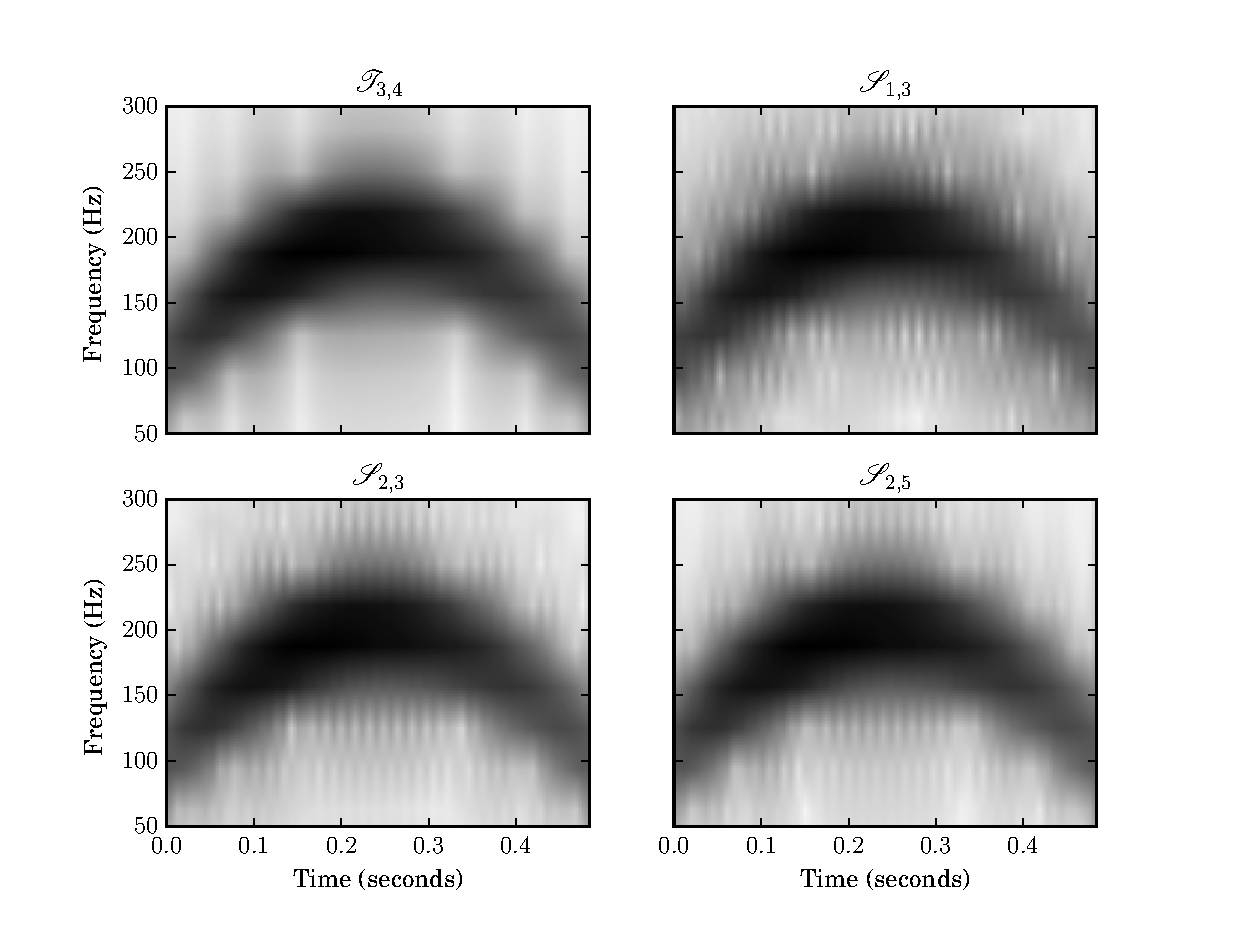
\includegraphics[width=\figwidthscale\textwidth]{plots/mq_mod_err_comp_all_spect.eps}
    \CaptionWithTitle{%
        \input{plots/mq_mod_err_comp_all_spect.txt}%
    }{
        Spectrograms of the true signal and estimated signals for the polynomial
        phase signal.
    \label{plot:mqmoderrorallspect}}
\end{figure}

\begin{figure}[!t]
    \centering
    \includegraphics[width=\figwidthscale\textwidth]{plots/mq_mod_err_comp_true_vs_est_err.eps}
    \CaptionWithTitle{%
        \input{plots/mq_mod_err_comp_true_vs_est_err.txt}%
    }{
        The power of the error when subtracting the original signal from the estimated
        signal. The local upper bound on the error was produced by connecting
        the local maxima in the error data.
    \label{plot:mqerrortruevsesterr}}
\end{figure}

\begin{figure}[!t]
    \centering
    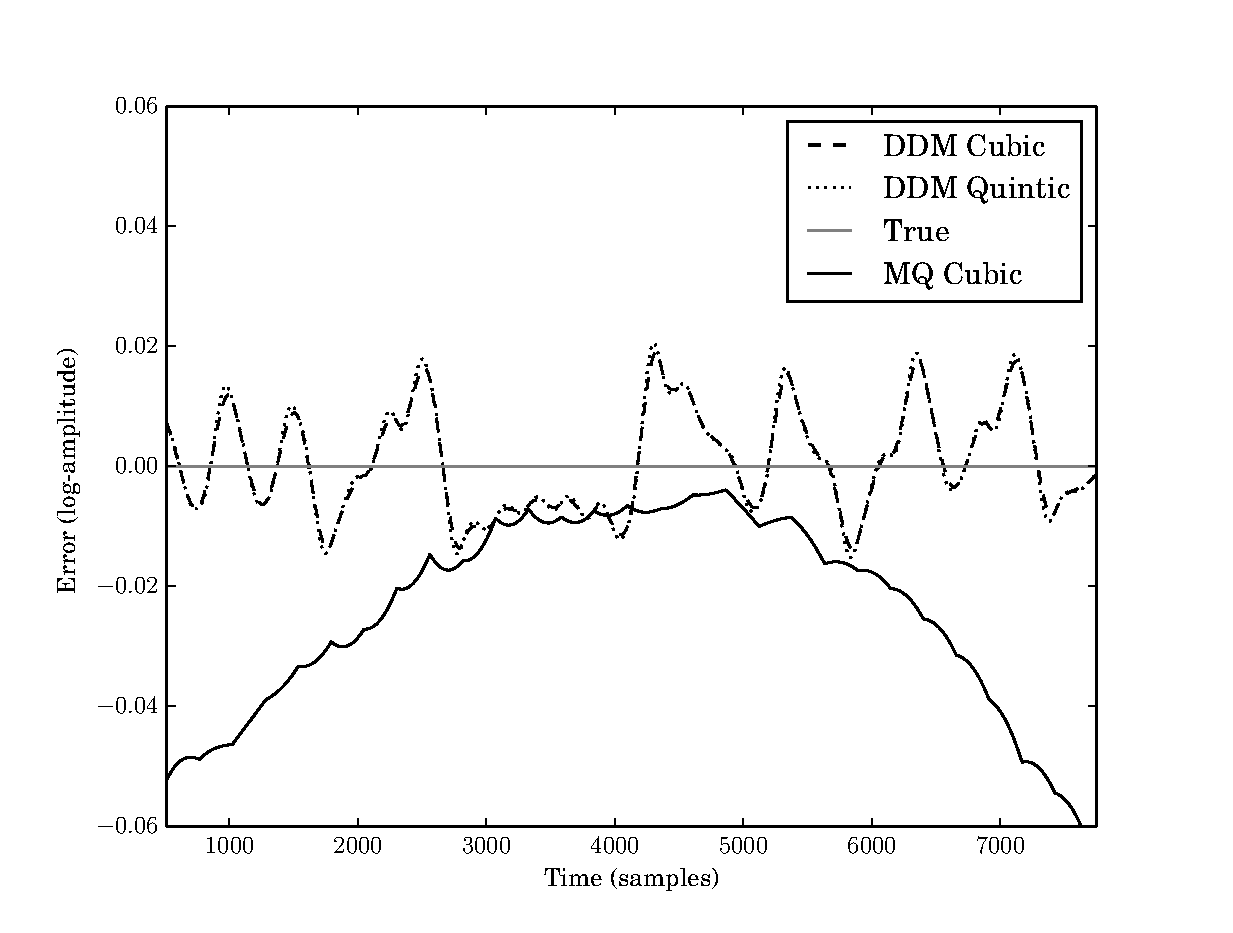
\includegraphics[width=\figwidthscale\textwidth]{plots/mq_mod_err_comp_logamp_err.eps}
    \CaptionWithTitle{%
        \input{plots/mq_mod_err_comp_logamp_err.txt}%
    }{This shows the error of the interpolated signals when compared
    with the original signal for the three proposed methods.
    \label{plot:mqmoderrcomplogamperr}}
\end{figure}

\begin{figure}[!t]
    \centering
    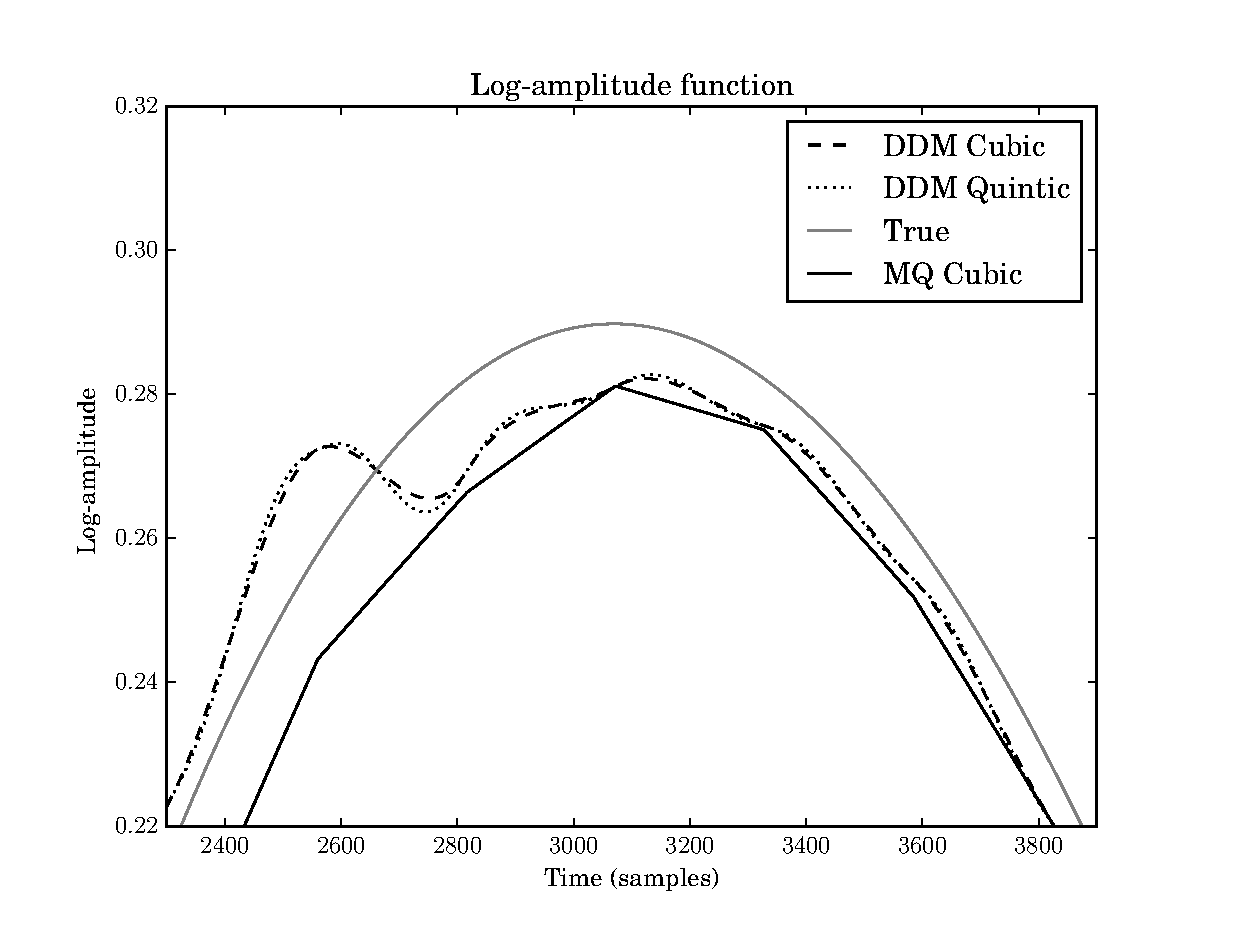
\includegraphics[width=\figwidthscale\textwidth]{plots/mq_mod_err_comp_logamp_func.eps}
    \CaptionWithTitle{%
        \input{plots/mq_mod_err_comp_logamp_func.txt}%
    }{This compares the original log-amplitude function with the
    interpolated log-amplitude functions. The log-amplitude functions are
    considered because these are the real part of the polynomial exponents in
    the complex sinusoid model.
    \label{plot:mqmoderrcomplogampfunc}}
\end{figure}

\begin{figure}[!t]
    \centering
    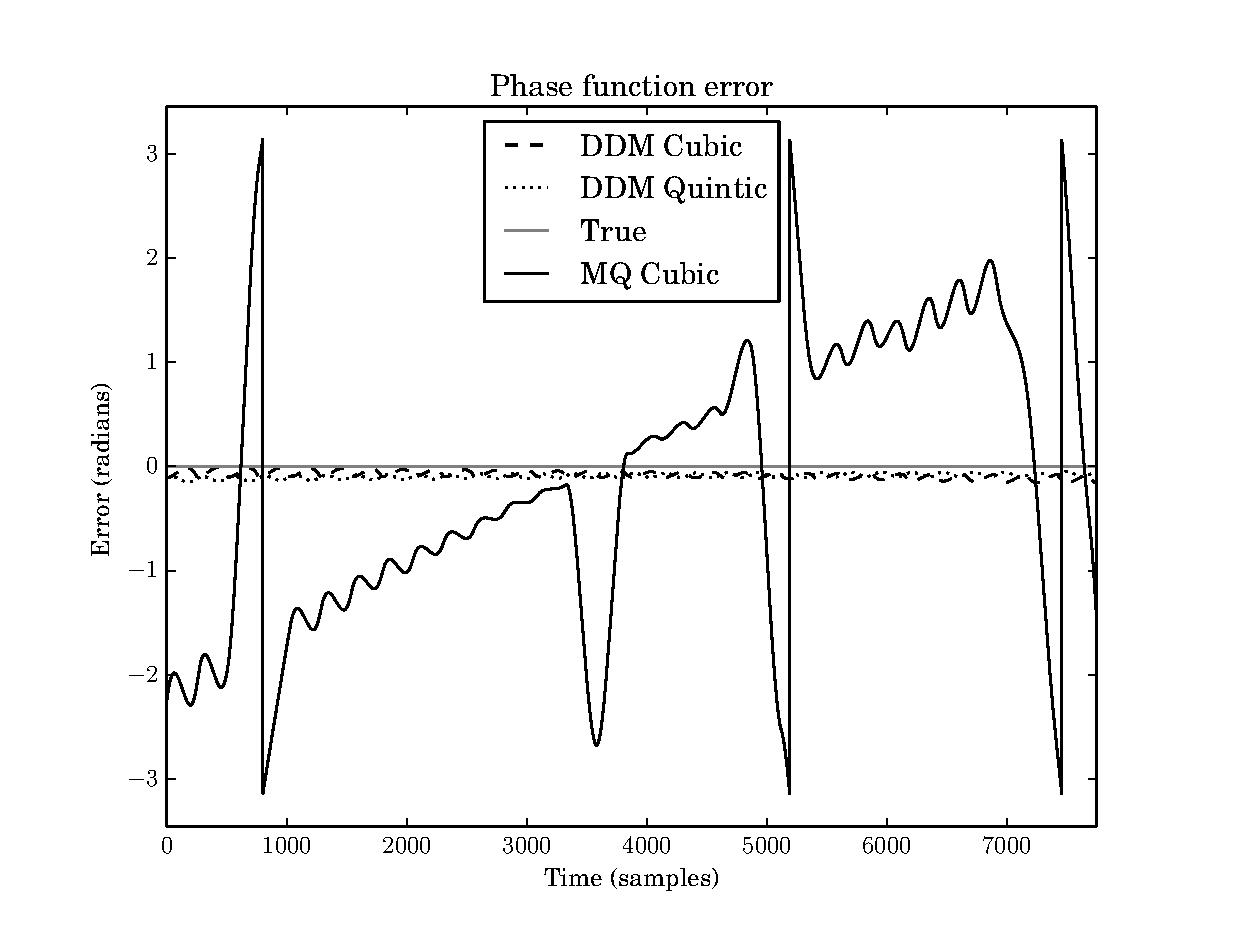
\includegraphics[width=\figwidthscale\textwidth]{plots/mq_mod_err_comp_phase_err.eps}
    \CaptionWithTitle{%
        \input{plots/mq_mod_err_comp_phase_err.txt}%
    }{This compares the theoretical phase function with the interpolated
        phase functions. The phase functions are considered because these are
        the imaginary part of the polynomial exponents in the complex sinusoidal
        model.  The errors are ``wrapped'' to lie between $-\pi$ and $\pi$. The
        errors stem from both the estimation of the phase and the interpolation
        of phase between analysis points. As a frequency modulated sinusoid is
        considered, it is not surprising that the stationary frequency
        assumption of the McAulay-Quatieri model exhibits the most errors.
    \label{plot:mqmoderrcompphaseerr}}
\end{figure}

%\begin{figure}[!t]
%    \centering
%    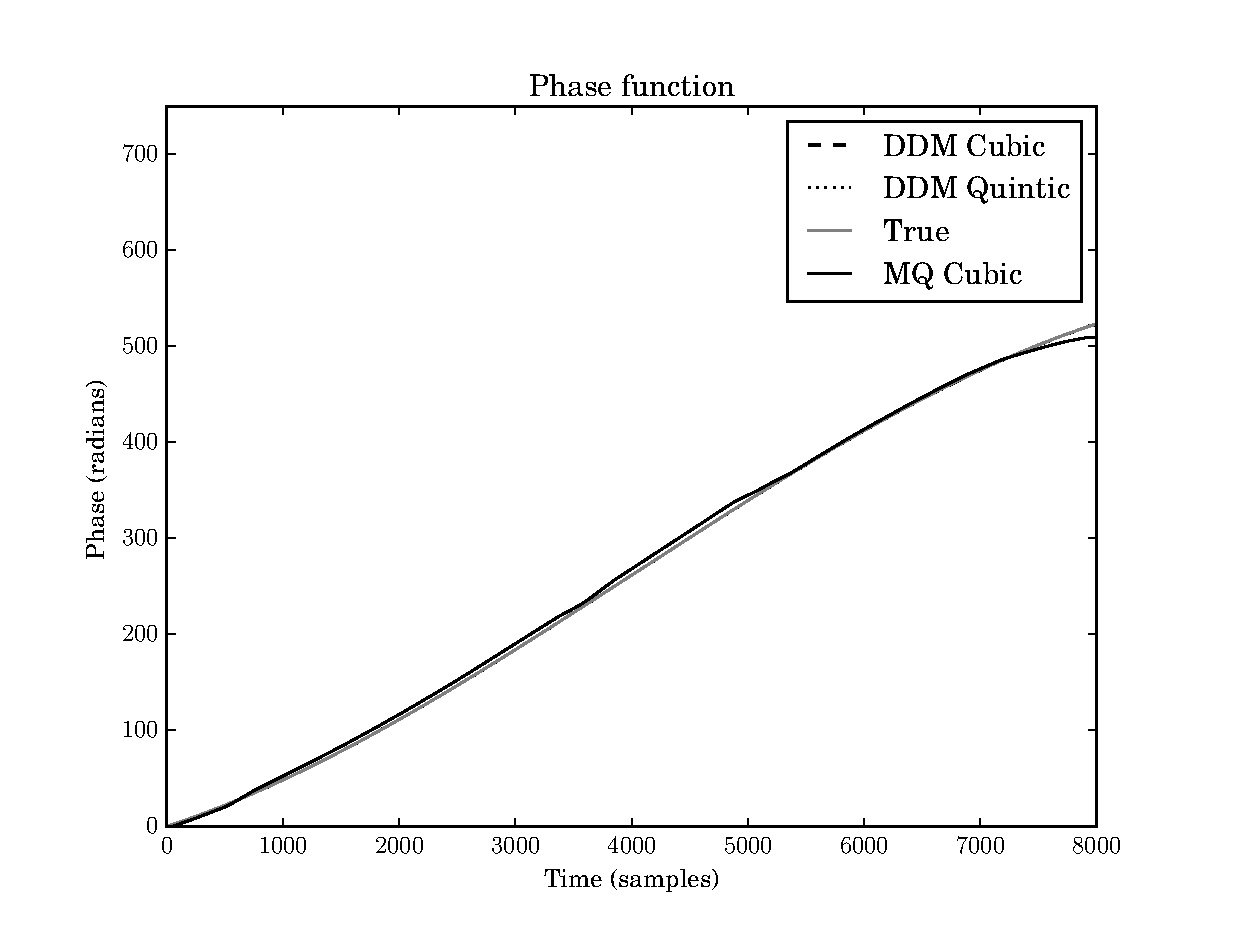
\includegraphics[width=\figwidthscale\textwidth]{plots/mq_mod_err_comp_phase_func.eps}
%    \caption{Error bound of polynomial evaluation using Horner's method. The
%    error bound is shown for the quintic phase and amplitude polynomials.
%    \label{plot:mqmoderrcompphasefunc}}
%\end{figure}

\subsection{Evaluation on sinusoid of exponential phase \label{sec:evalexpphase}}

The previous evaluation of this analysis-synthesis system was on a sinusoid with
small order polynomial phase. In the cases where we observed overfitting, the
polynomial used for synthesis was of higher order than the true underlying one
--- the interpolating polynomials were more times differentiable than the true
polynomial. We propose evaluating the system on an infinitely differentiable and
analytic phase function. The rationale behind this stems from the definition of
an analytic function: one whose power series representation (a polynomial)
converges to the function as the number of terms approches infinity. What this
means is, in the region of convergence, the larger the number of terms in the
approximating polynomial, the better the approximation to the true underlying
function. The exponential function
\[
    y=\exp(x), x,y \in \mathbb{R}
\]
is one such function whose power series is
\[
    \exp(x)=\sum_{n=0}^{\infty} \frac{x^{n}}{n!}
\]
To find the radius of convergence, we use the ratio test
\[
    \lim_{n \rightarrow \infty} \frac{|1/n!|}{|1/(n+1)!|} = \lim_{n \rightarrow \infty} n = \infty
\]
i.e., the power series of the exponential function converges everywhere and so
using more terms of its power series will improve its approximation for
any $x \in \mathbb{R}$.

The exponential function arises in music. In 12-tone equal temperament tuning,
to find the frequency $f_{1}$ of a pitch $b$-semitones away from the frequency
$f_{0}$ we compute
\[
    f_{1}=f_{0}2^{\frac{b}{12}}=f_{0}\exp(\log(2)\frac{b}{12})
\]
So a linear transition from pitch $b_{0}$ to $b_{1}$ is an exponential change in
frequency. This could be observed in recordings of performances of the
\textit{portamento} gesture.

We synthesize a sinusoid  of length $N$ samples with exponential phase and use
the same analysis system as in Section~\ref{sec:evalcubicphase} to evaluate the
synthesis accuracy for piece-wise interpolating polynomials of cubic and quartic
order for phase. The signal $x$ is defined
\[
    x(n) = \exp(\frac{2\pi f_{0}}{\log(2)c_{1}}\exp(j(c_{1}n + c_{0})))
\]
with
\[
    c_{0} = \log(2)\frac{b_{0}}{12}
\]
and
\[
    c_{1}= \log(2)\frac{b_{1}}{12N}
\]
i.e., a signal starting at pitch $b_{0}$ with frequency $f_{0}$ and arriving at
pitch $b_{1}$ in $N$ samples. We keep the amplitude of the signal constant in
this evalutation as we are interested in the accuracy of the phase
reconstruction. The same proceduare as in
Section~\ref{sec:evalcubicphase} is used to estimate the parameters of
piece-wise interpolating phase polynomials. We can see in
Figure~\ref{plot:mqexperrortruevsesterr} that the resynthesis accuracy is
greater for higher order polynomials. Spectrograms of the original and estimated
signals are plotted in Figure~\ref{plot:mqexperrorallspect}.


\begin{figure}[!t]
    \centering
    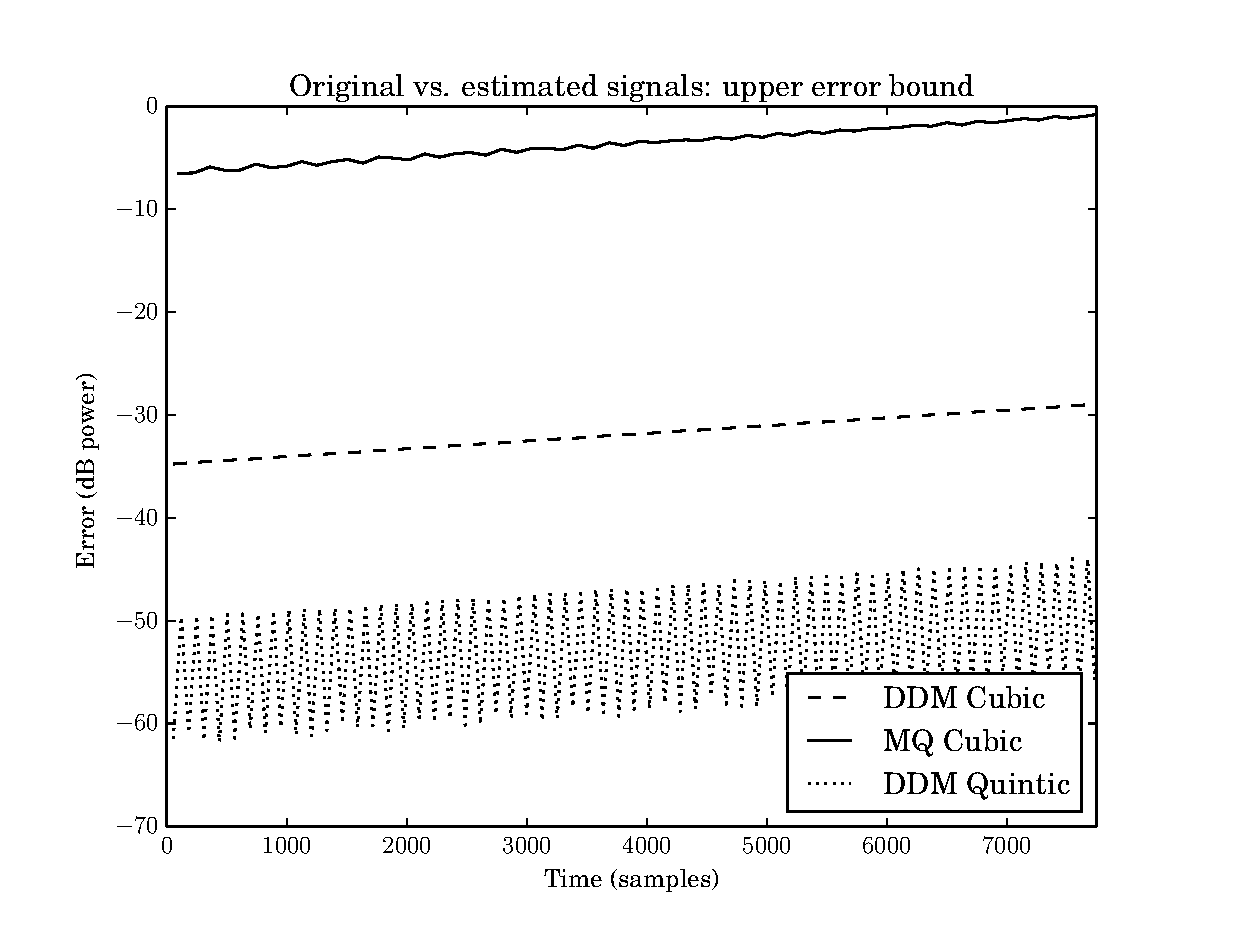
\includegraphics[width=\figwidthscale\textwidth]{plots/mq_exp_err_comp_true_vs_est_err.eps}
    \CaptionWithTitle{%
        \input{plots/mq_exp_err_comp_true_vs_est_err.txt}%
    }{
        The power of the error when subtracting the original signal from the
        estimated signal for the signals of exponential phase. The local upper
        bound on the error was produced by connecting the local maxima in the
        error data.
    \label{plot:mqexperrortruevsesterr}}
\end{figure}

\begin{figure}[!t]
    \centering
    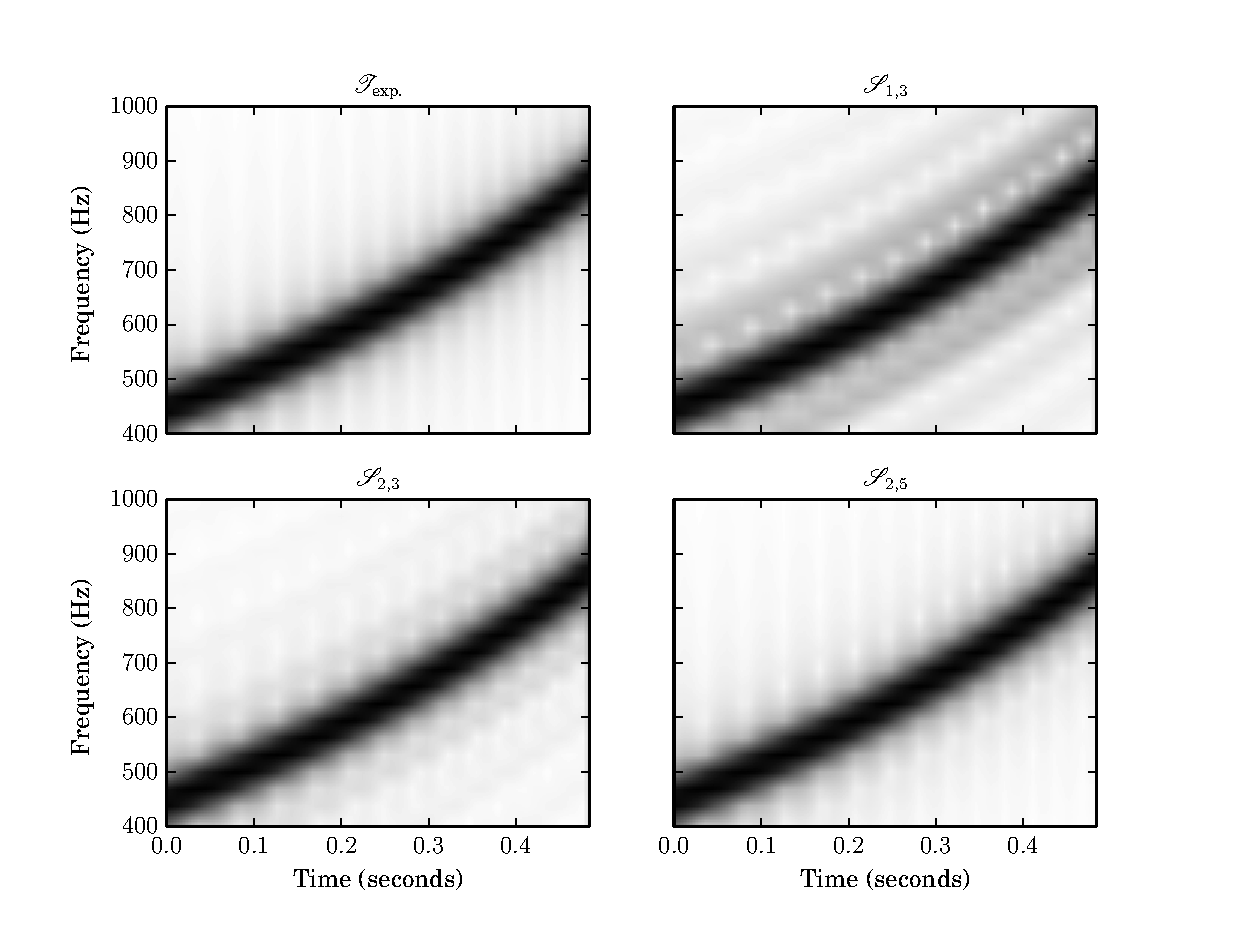
\includegraphics[width=\figwidthscale\textwidth]{plots/mq_exp_err_comp_all_spect.eps}
    \CaptionWithTitle{%
        \input{plots/mq_exp_err_comp_all_spect.txt}%
    }{
        Spectrograms of the true signal and estimated signals for the
        exponential phase signal.
    \label{plot:mqexperrorallspect}}
\end{figure}

\section{Conclusion}

\subsection{Polynomial phase function}

Out of the three proposed methods it appears that the modified cubic
interpolation method works superiorly for the signal model considered. We obseve
overfitting by the higher-order quintic model in
Figure~\ref{plot:mqmoderrcomplogampfunc}, compromising the accuracy of
resynthesis.  Even the proposed cubic model shows some overfitting in this case.
This is consistent with the results of \cite{girin2003comparing}. From
Figure~\ref{plot:mqmoderrcompphaseerr} it is clear that the DDM based methods
provide superior estimation of the phase function --- this is not the case for
the log-amplitude function. Depending on the underlying signal, perhaps better
results can be obtained by postulating a lower-order amplitude function and
higher-order phase function. The possibility of errors arising from numerical
accuracy when evaluating the quintic polynomials has been ruled out.  We
evalutated these polynomials using an implementation of Horner's method that
keeps track of the error bound \cite[p.~95]{higham2002accuracy}: the errors are
negligible, see Figure~\ref{plot:mqmodquinticpolyevalerr} for the results.

\begin{figure}[!t]
    \centering
    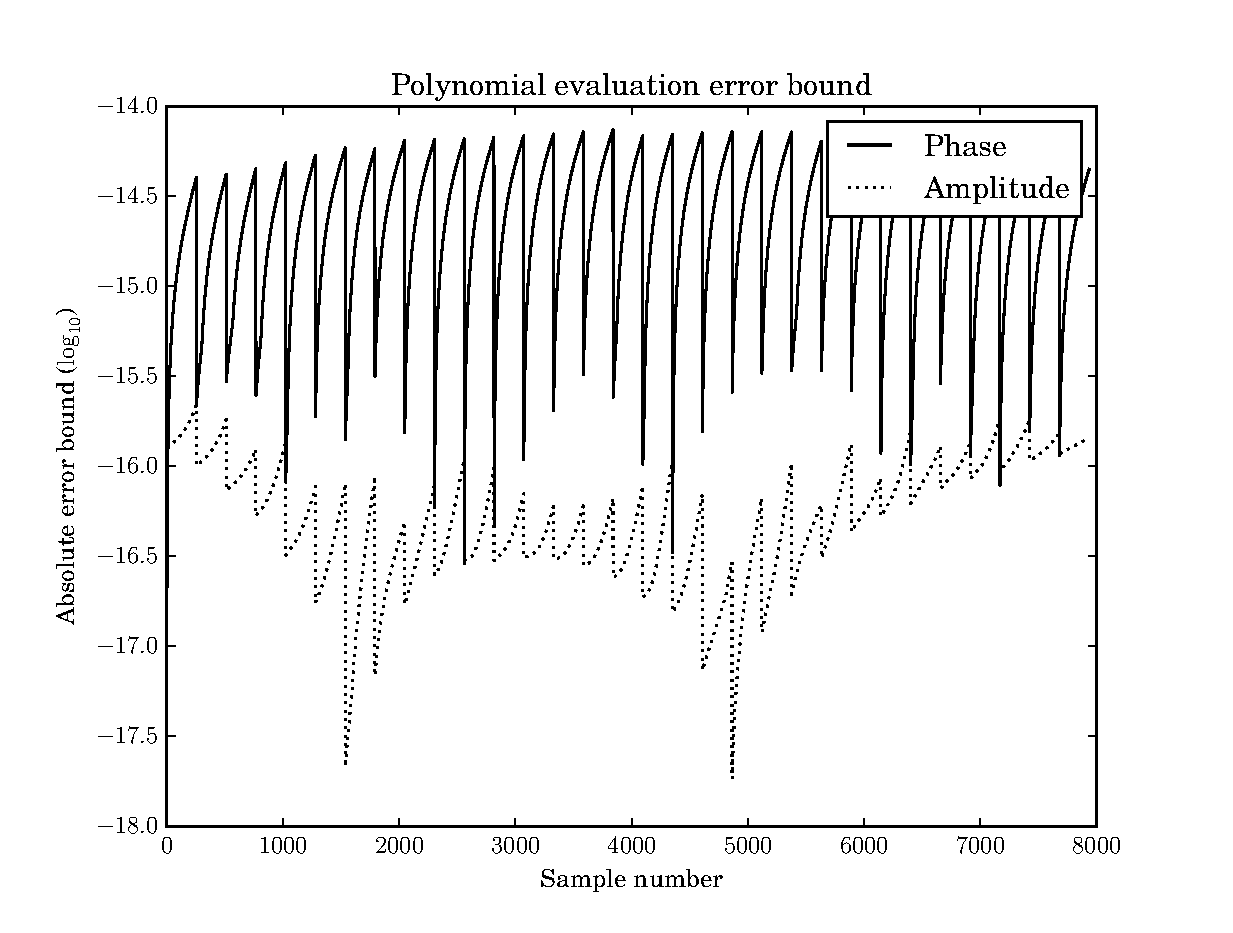
\includegraphics[width=\figwidthscale\textwidth]{plots/mq_mod_quintic_poly_eval_err.eps}
    \CaptionWithTitle{%
        \input{plots/mq_mod_quintic_poly_eval_err.txt}%
    }{The error bound in evaluating the quintic amplitude and phase
    polynomials using Horner's method. This plot was produced by plotting only
    the local maxima of the error bound data in order to reduce the plot's
    range.\label{plot:mqmodquinticpolyevalerr}}
\end{figure}

\subsection{Exponential phase function}

The quintic interpolation, the polynomial of highest order, performs the most
accurate resynthesis. This is consistent with the analytic property of the
exponential function and an encouraging result as it suggests arbitrary analytic
phase functions can be approximated with arbitrary accuracy simply by increasing
the order of the interpolating polynomials. Many models of musical gestures
involve such functions, apart from the portamento gesture modeled by an
exponential phase function, vibrato can be modeled as a sinusoid with sinusoidal
phase \cite{maher1990investigation}. The DDM-based analysis system combined with
the higher order polynomial phase synthesis system presented here allow for
accurate modeling of these gestures.
